\documentclass[supercite]{Experimental_Report}

\title{~~~~~~计算机视觉专题实验报告~~~~~~}
\author{崔昊阳}
\school{计算机科学与技术学院}
\classnum{CS2104}
\stunum{U202115415}
\instructor{刘康}
\date{2024年1月13日}

\usepackage{algorithm, multirow}
\usepackage{algpseudocode}
\usepackage{amsmath}
\usepackage{amsthm}
\usepackage{framed}
\usepackage{mathtools}
\usepackage{subcaption}
\usepackage{xltxtra}
\usepackage{bm}
\usepackage{tikz}
\usepackage{tikzscale}
\usepackage{pgfplots}
\usepackage{listings}
\usepackage{newtxmath}
\lstset{
    backgroundcolor = \color{white},    % 背景色
    basicstyle = \small\ttfamily,           % 基本样式 + 小号字体
    rulesepcolor= \color{white},             % 代码块边框颜色
    breaklines = true,                  % 代码过长则换行
    numbers = left,                     % 行号在左侧显示
    numberstyle = \small,               % 行号字体
    keywordstyle = \color{blue}\bfseries,      % 关键字颜色
	identifierstyle=\color{purple}, 		% 标识符颜色
    commentstyle =\color{green},        % 注释颜色
    stringstyle = \color{green},          % 字符串颜色
    frame = None,                  % 用(带影子效果)方框框住代码块
    showspaces = false,                 % 不显示空格
    columns = flexible,                    % 字间距固定
}

\pgfplotsset{compat=1.16}

\newcommand{\cfig}[3]{
  \begin{figure}[H]
    \centering
    \includegraphics[width=#2\textwidth]{images/#1.tikz}
    \caption{#3}
    \label{fig:#1}
  \end{figure}
}

\newcommand{\sfig}[3]{
  \begin{subfigure}[b]{#2\textwidth}
    \includegraphics[width=\textwidth]{images/#1.tikz}
    \caption{#3}
    \label{fig:#1}
  \end{subfigure}
}

\newcommand{\xfig}[3]{
  \begin{figure}[H]
    \centering
    #3
    \caption{#2}
    \label{fig:#1}
  \end{figure}
}

\newcommand{\rfig}[1]{\autoref{fig:#1}}
\newcommand{\ralg}[1]{\autoref{alg:#1}}
\newcommand{\rthm}[1]{\autoref{thm:#1}}
\newcommand{\rlem}[1]{\autoref{lem:#1}}
\newcommand{\reqn}[1]{\autoref{eqn:#1}}
\newcommand{\rtbl}[1]{\autoref{tbl:#1}}

\algnewcommand\Null{\textsc{null }}
\algnewcommand\algorithmicinput{\textbf{Input:}}
\algnewcommand\Input{\item[\algorithmicinput]}
\algnewcommand\algorithmicoutput{\textbf{Output:}}
\algnewcommand\Output{\item[\algorithmicoutput]}
\algnewcommand\algorithmicbreak{\textbf{break}}
\algnewcommand\Break{\algorithmicbreak}
\algnewcommand\algorithmiccontinue{\textbf{continue}}
\algnewcommand\Continue{\algorithmiccontinue}
\algnewcommand{\LeftCom}[1]{\State $\triangleright$ #1}

\newtheorem{thm}{定理}[section]
\newtheorem{lem}{引理}[section]

\colorlet{shadecolor}{black!15}

\theoremstyle{definition}
\newtheorem{alg}{算法}[section]

\def\thmautorefname~#1\null{定理~#1~\null}
\def\lemautorefname~#1\null{引理~#1~\null}
\def\algautorefname~#1\null{算法~#1~\null}

\begin{document}

\maketitle

\clearpage

\pagenumbering{Roman}

\tableofcontents[level=2]

\clearpage

\pagenumbering{arabic}

\section{实验总述}

在本次实验中,我选择了\textbf{任务二\quad 专题实验报告}。
我完成了全部的基础要求,具体如下。
\begin{enumerate}
	\item 复现了 GradCAM++ 代码
	\item 复现了 ScoreCAM 代码
	\item 获取了 LIME 库的源代码并进行了改写,使之可以整合进实验代码中
	\item 对比了三种方法的可解释性分析结果,分析了各自的优缺点
\end{enumerate}

在完成所有的基础要求的同时,我还对实验进行了一些扩展。
我补充了从理论上解释 CAM 算法的有效性的 XGradCAM 算法和 CAM 算法在医学图像处理上的应用:HiResCAM。同时还讨论了 2 种热力图平滑方法。
\textbf{扩展内容}包括:
\begin{enumerate}
	\item 复现了 XGradCAM 代码
	\item 复现了 HiResCAM 代码
	\item 实现了 CAM 可解释性分析中的两种平滑方法:测试时增强平滑(Augmentation Smooth)和主成分降噪平滑(Eigen Smooth)并进行了对比分析
	\item 在报告中展现了自己对每种方法的理解或对方法存在的缺陷的思考、改进
\end{enumerate}

\section{数据集读取}
本次实验中的数据处理部分相对简单,仅需要读取 3 张用于测试的图片。
我们编写了一个支持迭代的数据集类,用于将 3 张用于测试的图片转换成可输入模型的形式。在实例化此类时,我们传入
测试集的地址。在每次迭代时,实例会读入对应的图像并将其转换成 Tensor 格式返回。具体代码如下。
\begin{lstlisting}
class PicDataset(Dataset):
"""
猫狗分类的 Dataset
:params data_path: 数据集路径
"""

def __init__(self, data_path: str):
    super().__init__()
    self.data_path = data_path
    self.data_info = os.listdir(self.data_path)
    self.transform = transforms.Compose([transforms.ToTensor()])

def __getitem__(self, index):
    img_path = os.path.join(self.data_path, self.data_info[index])
    img = self.transform(Image.open(img_path))
    return img

def __len__(self):
    return len(self.data_info)
\end{lstlisting}

\section{可解释性分析算法}
可解释性是指以可理解的方式向人类提供解释的能力。而深度学习模型的可解释性是指解释和理解模型如何做出预测和决策。
可解释性分析算法可以揭示模型的行为,并提供对模型预测的解释。
深度学习模型的可解释性具有重要意义,它可以帮助我们提高模型的可靠性,发现模型的缺点以及满足一些法律、伦理上的要求。

在本章中,我们将介绍本次实验使用的所有可解释性算法。
它们可以分为两大类:LIME 和 CAM。其中,CAM 算法下又有 4 种改进算法:GradCAM++,XGradCAM,ScoreCAM 以及 HiResCAM。
我们首先介绍 LIME 可解释性算法,接着介绍 CAM 可解释性算法,然后依次介绍CAM 算法下的 4 种改进算法,最后我们还会介绍 2 种平滑方法。  
\subsection{LIME}

LIME 算法\cite{LIME} 是 Marco Tulio Ribeiro 等人于 2016 年提出的一种局部可解释性模型算法。
该算法主要是用在文本类与图像类的模型中。LIME 采取以样本代替总体的思路,
可以以可理解的方式解释任何类型的模型的预测结果。

以图\ref{LIME算法大致流程}的简单非线性模型为例,LIME 的大致流程如下。
\begin{figure}[H]
	\begin{center}
		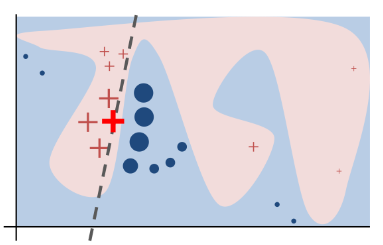
\includegraphics[scale=1.0]{../images/LIME算法大致流程.png}
		\caption{LIME算法的简单例子}
		\label{LIME算法大致流程}
	\end{center}
\end{figure}

\begin{enumerate}
	\item 选择一个待解释的样本(图中加粗的红色加号点)
	\item 对这个样本进行扰动,获得在其附近的多个扰动数据点(图中若干红色加号点和蓝色圆点)
	\item 根据扰动数据点与样本的接近程度对其进行加权
	\item 在上述数据点形成的数据集上训练一个可解释的线性模型
	\item 通过可解释的线性模型来解释难以解释的复杂模型的一个局部
\end{enumerate}

具体而言,假设我们选取待解释样本为 $x$,其邻域为 $\pi_x$,待解释的复杂模型为 $f$,需要逼近 $f$ 的可解释模型为 $g$。
则 LIME 需要最小化的优化目标可以形式化地表示成
\begin{equation}
	\epsilon(x)=\underset{g\in G}{argmin} L(f, g, \pi_x)+\Omega(g)
\end{equation}

其中,$G$ 是所有可能的可解释模型的集合,$\Omega(\cdot)$ 定义了可解释性模型的复杂程度。
$L(\cdot)$ 是原始模型和可解释模型预测的不相似程度。实际上,$\Omega(\cdot)$ 的值在算法开始前指定并保持不变,
算法仅优化原始模型和可解释模型预测的相似程度。

根据上述公式,我们首先需要确定可解释模型 $g$。在本次实验中,我们选择岭回归模型作为可解释模型。
接着,我们需要对图像进行扰动。我们将待解释的图像分割成若干超像素,接着通过将某些超像素中的所有像素进行平均值池化来进行扰动。
然后,我们确定衡量两模型相似程度的距离函数$L(\cdot)$。我们使用余弦相似度来衡量两模型预测结果之间的相似程度。
最后,我们即可训练出一个岭回归模型,并据此判定哪一块超像素对图像分类结果的判定较为重要。


\subsection{CAM}
CAM 算法(类激活映射算法)\cite{CAM}是由 Bolei Zhou 等人于 2016 年提出的,用于可视化卷积神经网络在图像分类任务中的关注区域的可解释性分析算法。
CAM 算法的大致流程如图\ref{CAM}所示,其具体过程如下。
\begin{figure}[H]
	\begin{center}
		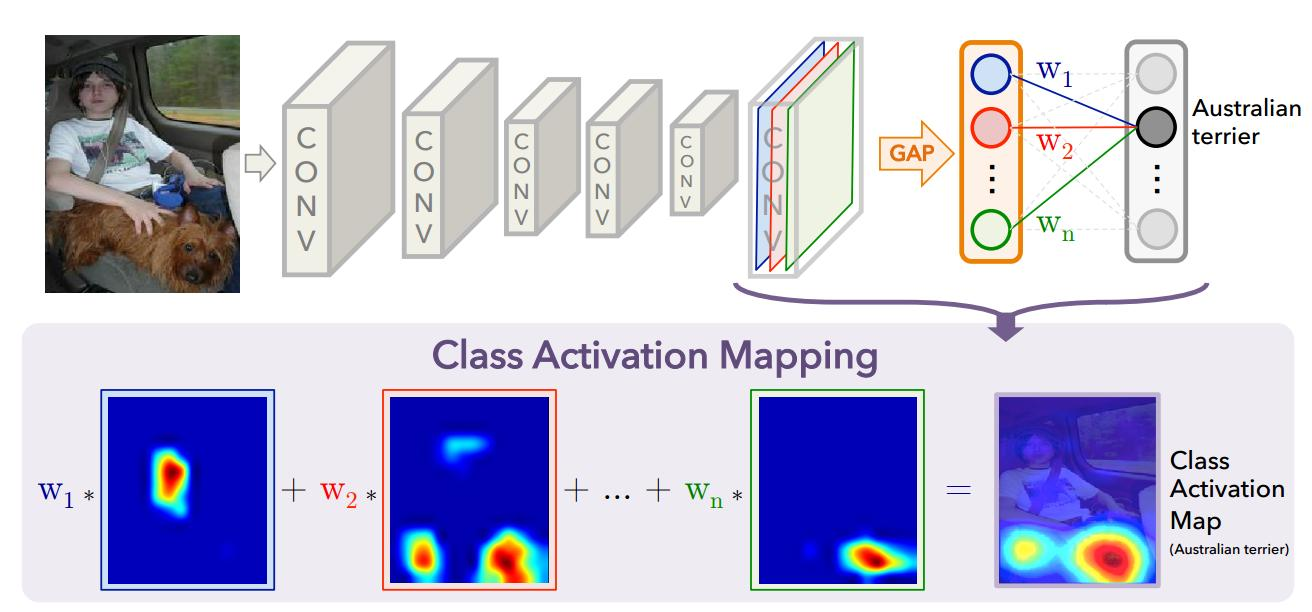
\includegraphics[scale=0.25]{../images/CAM算法结构图.png}
		\caption{CAM 算法结构图}
		\label{CAM}
	\end{center}
\end{figure}

首先,CAM 算法将卷积神经网络的最后一层的输出进行全局平均池化(GAP)操作,获取在最后一个卷积层的各单元特征图的空间平均值。
\begin{equation}
  P_k=\frac{1}{N^2}\sum_{i=1}^{N}\sum_{j=1}^{N}A_k(i, j)
\end{equation}

其中,$A_k(i, j)$ 是最后一个卷积层上的第 $k$ 个通道的特征图,$P_k$ 是第 $k$ 个通道的全局平均池化结果,$N$ 是图像的分辨率。

接着,我们对每个通道的全局平均池化结果进行加权平均,得到每个分类的 logit。
\begin{equation}
  L_c=\sum_{k=1}^{K}w_k^cP_k
\end{equation}

其中,$w_k^c$ 是分类 $c$ 在第 $k$ 个通道上的权重,$P_k$ 是第 $k$ 个通道上的全局平均池化值,$K$ 是输入图像的通道总数。

然后使用 \texttt{softmax} 函数得到每个类别的概率分布并选择概率最大的类别作为目标类。训练完成后,我们将得到一组合适的权重 $w$。

最后,将训练好的权重与最后一层卷积的图像进行加权求和后经过 ReLU 激活函数,并上采样到和原始图像一样的大小,即可得到 CAM 热力图。
\begin{eqnarray}
  CAM_c(i, j)=max\{\sum_{k=1}^{K}w_k^cA_k(i, j), 0\}
\end{eqnarray}

其中,$w_k^c$ 是分类 $c$ 在第 $k$ 个通道上的权重,$A_k(i, j)$是最后一个卷积层上的第 $k$ 个通道的特征图,$K$ 是输入图像的通道总数。

CAM 算法可以提供直观的模型预测解释。但是,CAM 算法也存在着诸多缺陷。
首先,CAM 只能分析最后一层卷积层输出,无法分析中间层。
其次,CAM 只适用于图像分类任务。上述两个缺点限制了 CAM 的应用范围。
最后,CAM 要求模型必须有 GAP 层,否则需要修改模型并重新训练,这降低了 CAM 算法的应用方便性。
因此,人们提出了基于 CAM 算法的许多改进算法。

\subsection{GradCAM++}
GradCAM++\cite{GradCAM++} 是对 GradCAM 算法的改进,它是由 Aditya Chattopadhyay 等人于 2018 年提出的。
GradCAM 等基于梯度的可视化方法有一定的局限性。例如,当一张图像存在多个同类物体时 GradCAM 热力图通常不能覆盖所有同类物体。
另外,对于单个物体,GradCAM 热力图通常也不能完整地覆盖整个物体。
GradCAM++ 算法的大致流程以及和 GradCAM 的对比如图\ref{GradCAM++}所示,其具体过程如下。
\begin{figure}[H]
	\begin{center}
		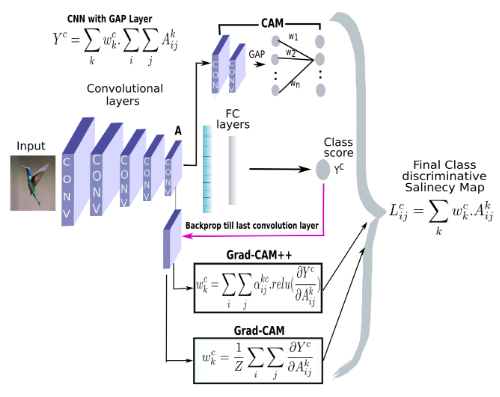
\includegraphics[scale=1.0]{../images/GradCAM++算法结构图.png}
		\caption{GradCAM++ 算法结构图}
		\label{GradCAM++}
	\end{center}
\end{figure}

首先,在存在 GAP 的卷积神经网络中,对于特定类别 c 的 logits $L_c$ 可以写成如下形式:
\begin{equation}
l^c=\sum_{k=1}^{K}w_k^c\sum_{i=1}^{N}\sum_{j=1}^{N}A_k(i,j)
\end{equation}

其中,$w_k^c$ 是各通道的权重,$A_k$ 是目标层的第 $k$ 通道的特征图,$K$ 是输入图像的通道总数,$N$ 是图像的分辨率。

接着,我们对梯度进行像素级的加权平均,获取各通道的权重。
\begin{equation}
w_k^c=\sum_{i=1}^{N}\sum_{j=1}^{N}\alpha_k^c(i,j)max\{\frac{\partial L^c}{\partial A_k(i, j)},0\}
\end{equation}

其中,$w_k^c$ 是各通道的权重,$\alpha_k^c$ 是类别 $c$ 在第 $k$ 个通道上的像素梯度加权系数,$L^c$ 是类别 $c$ 的 logits,$A_k$ 是目标层的第 $k$ 通道的特征图,$N$ 是图像的分辨率。

将上两式联立可得。
\begin{equation}
L^c=\sum_{k=1}^{K}\{\sum_{a=1}^{N}\sum_{b=1}^{N}\alpha_k^c(a,b)max\{\frac{\partial L^c}{\partial A_k(a,b)},0\}\}[\sum_{i=1}^{N}\sum_{j=1}^{N}A_k(i,j)]
\end{equation}

将上式恒等变换,我们可以分别求解出 $\alpha_k^c$ 和 $w_k^c$。
\begin{equation}
	\left\{
		\begin{aligned}
			\alpha_k^c&=\frac{\frac{\partial^2 L^c}{\partial A_k^2(i, j)}}{2\frac{\partial^2 L^c}{\partial A_k^2(i, j)}+\sum_{a=1}^{N}\sum_{b=1}^{N}A_k(a,b)\{\frac{\partial^3 L^c}{\partial A_k^3(i, j)}\}}\\
			w_k^c&=\sum_{i=1}^{N}\sum_{j=1}^{N}\frac{\frac{\partial^2 L^c}{\partial A_k^2(i, j)}}{2\frac{\partial^2 L^c}{\partial A_k^2(i, j)}+\sum_{a=1}^{N}\sum_{b=1}^{N}A_k(a,b)\{\frac{\partial^3 L^c}{\partial A_k^3(i, j)}\}}max\{\frac{\partial L^c}{\partial A_k(i, j)},0\}
		\end{aligned}
	\right.
\end{equation}

最后,我们将各通道的特征图加权求和并经 ReLU 去除负值,得到最终的类激活映射。
\begin{equation}
GCAMpp_c(i, j)=max\{\sum_{i=1}^{K}w_k^cA_k(i, j), 0\}
\end{equation}

其中,$w_k^c$ 是分类 $c$ 在第 $k$ 个通道上的权重,$A_k$ 是目标层的第 $k$ 通道的特征图,$K$ 是输入图像的通道总数。

GradCAM++ 算法解决了 GradCAM 中存在的难以检测全部同类物体和难以完全覆盖单一物体的问题。
该算法还在图像描述生成、动作识别等任务的解释上具有优势。
但是,GradCAM++ 同样存在着缺陷:
GradCAM++ 缺乏明确的理论支持,例如,为什么可以使用像素级的加权平均作为每个特征的权重。
因此,人们提出了 XGradCAM 对其进行了改进。

\subsection{XGradCAM}
XGradCAM\cite{XGradCAM} 是对 GradCAM 和 GradCAM++ 等算法的改进,它是由 Ruigang Fu 等人于 2020 年提出的。
XGradCAM 是一种基于公理的 CAM 可解释性算法,这使得此可视化方法更具可靠性和理论性。
XGradCAM 算法的大致流程如图\ref{XGradCAM}所示,其具体过程如下。
\begin{figure}[H]
	\begin{center}
		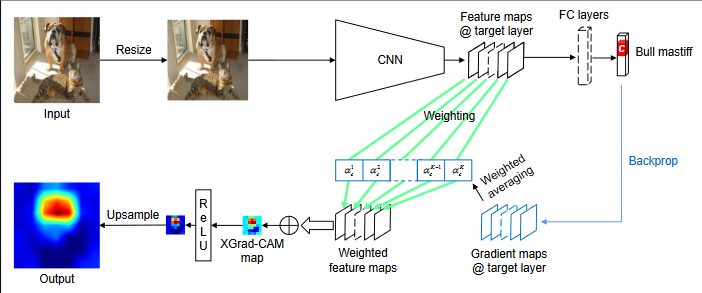
\includegraphics[scale=0.8]{../images/XGradCAM算法结构图.png}
		\caption{XGradCAM 算法结构图}
		\label{XGradCAM}
	\end{center}
\end{figure}

首先,我们提出可解释性算法需要满足的 4 个公理:连续性、实现不变性、敏感性和一致性。假设待解释的模型为 $m$,其输入为 $x\in \vmathbb{R}^d$。$f(x,m)$ 是 $m$ 中输入向输出的映射,$R(x,m)$ 是 $m$ 的解释。

连续性要求对于两个几乎相同的输入,模型输出几乎相同,那么相应的解释也应该是几乎相同的。
\begin{equation}
	R(x,m)\approx R(x+\epsilon,m)
\end{equation}

其中,$\epsilon$ 是一个小的扰动。

实现不变性要求对具有相同输入的功能等效模型产生相同的解释。
\begin{equation}
	R(x,m_1)=R(x,m_2)
\end{equation}

其中,$m_1$ 和 $m_2$ 是等效的模型。(对任意相同的输入产生相同的输出)

敏感性要求解释的每个响应应该等于去除输入的相应特征所引起的输出变化。
\begin{equation}
	R_i(x,m)=f(x,m)-f(x\backslash x_i,m)
\end{equation}

其中,$x\backslash x_i$ 指原始输入中的第 $i$ 个特征被屏蔽后的输入。

一致性要求解释响应的总和应该与模型输出的大小相匹配。
\begin{equation}
	f(x,m)=\sum_{i=1}^{d}(R_i(x,m))
\end{equation}

对于一个 CAM 模型,我们的优化目标是使其尽可能具有敏感性和一致性,即使得如下优化目标$\phi(w_k^c)$最小。
\begin{equation}
	\phi(w_k^c)=\sum_{k=1}^{K}|L^c(A)-L^c(A\backslash A_k)-\sum_{i=1}^{N}\sum_{j=1}^{N}w_k^cA_k(i,j)|+|L^c(A)-\sum_{i=1}^{N}\sum_{j=1}^{N}(\sum_{k=1}^{K}w_k^cA_k(i,j))|
\end{equation}

其中,第一项表示 CAM 算法对敏感性的偏离程度,第二项表示 CAM 算法对一致性的偏离程度。
$w_k^c$ 是分类 $c$ 在第 $k$ 个通道上的权重,$L^c$ 是第 $c$ 通道上的 logits,$A_k$ 是目标层的第 $k$ 通道的特征图,$K$ 是输入图像的通道总数,$N$ 是图像的分辨率。

经过推导,可知上式有一个近似的闭式解。
\begin{equation}
	\left\{
		\begin{aligned}
			\alpha_k^c&=\sum_{i=1}^{N}\sum_{j=1}^{N}(\frac{A_k(i,j)}{\sum_{a=1}^{N}\sum_{b=1}^{N}A_k(a,b)}\frac{\partial L_c}{\partial A_k(x,y)})\\
			XGCAM_c(i,j)&=\sum{i=1}^{K}(\alpha_k^cA_k(i,j))
		\end{aligned}
	\right.
\end{equation}

以上即是 XGradCAM 的计算方法。

XGradCAM 为 CAM 算法提供了清晰的数学解释,填补了 CAM 可视化方法本身在可解释性方面的空白。
同时从公理的角度给出了 GradCAM,GradCAM++ 算法为何有效的合理解释。
但是,由于梯度的饱和性、梯度本身的不稳定性(局部的梯度受噪声影响很大)以及梯度消失的影响,
基于梯度的 CAM 方法具有一些难以克服的问题,例如在GradCAM中获得较高权重的特征图,在网络中的响应很低,而部分权重较低的特征图,则获得到了很高的置信度。
因此,人们提出了 ScoreCAM 使得 CAM 算法不再依赖于梯度。

\subsection{ScoreCAM}
ScoreCAM\cite{ScoreCAM} 是对基于梯度的 CAM 算法的改进,它是由 Haofan Wang 等人于 2020 年提出的。
ScoreCAM 算法首次摆脱了对于梯度的依赖,使用模型对于特征图的全局置信分数来衡量线性权重。
ScoreCAM 算法的大致流程如图\ref{ScoreCAM}所示,其具体过程如下。
\begin{figure}[H]
	\begin{center}
		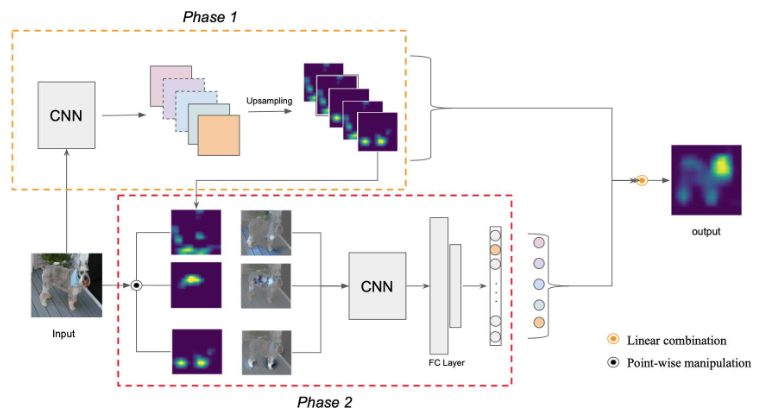
\includegraphics[scale=0.8]{../images/ScoreCAM算法结构图.png}
		\caption{ScoreCAM 算法结构图}
		\label{ScoreCAM}
	\end{center}
\end{figure}

首先,定义置信度提升。假设输入到输出的映射为 $f(\cdot)$,输入为 $x\in \vmathbb{R}^n$,则 $x_i$ 对输出 $y$ 的贡献 $c_i$
可表示成
\begin{equation}
	c_i=f(x\circ H_i)-f(x)
\end{equation}

其中,$H_i\in \vmathbb{R}^n$ 且 $H_i[j]=\vmathbb{I}[i=j]$,$\circ$ 表示哈达玛积。

接着,我们定义通道级置信度提升(CIC)。仿照上式,有
\begin{equation}
	C(A_k)=f(x\circ H_k)-f(x)
\end{equation}

其中,$A_k$ 是第 $k$ 通道的特征图矩阵。
\begin{equation}
	H_k=\frac{Up(A_k)-min\{Up(A_k)\}}{max\{Up(A_k)\}-min\{Up(A_k)\}}
\end{equation}

$Up(\cdot)$ 是上采样函数。

最后,我们将各通道的特征图加权求和并经 ReLU 去除负值,得到最终的类激活映射。
\begin{equation}
	SCAM_c(i,j)=max\{\sum_{i=1}^{K}C(A_k)A_k(i,j), 0\}
\end{equation}

其中,$A_k$ 是第 $k$ 通道的特征图矩阵,$K$ 是通道总数。

ScoreCAM 去除了对梯度的依赖,摆脱了梯度本身的问题对模型可解释性算法的不良影响,且具有更合理的权重表示。

\subsection{HiResCAM}
HiResCAM\cite{HiResCAM} 是一种用于医学图像处理领域的可解释性算法。它是由 Rachel Lea Draelos 等人于 2020 年提出的。
HiResCAM 算法主要应用于 3D CT 图像上识别病灶区域的模型的可解释性分析,也可应用于 2D 的自然图像。
HiResCAM 算法的大致流程如图\ref{HiResCAM}所示。
\begin{figure}[H]
	\begin{center}
		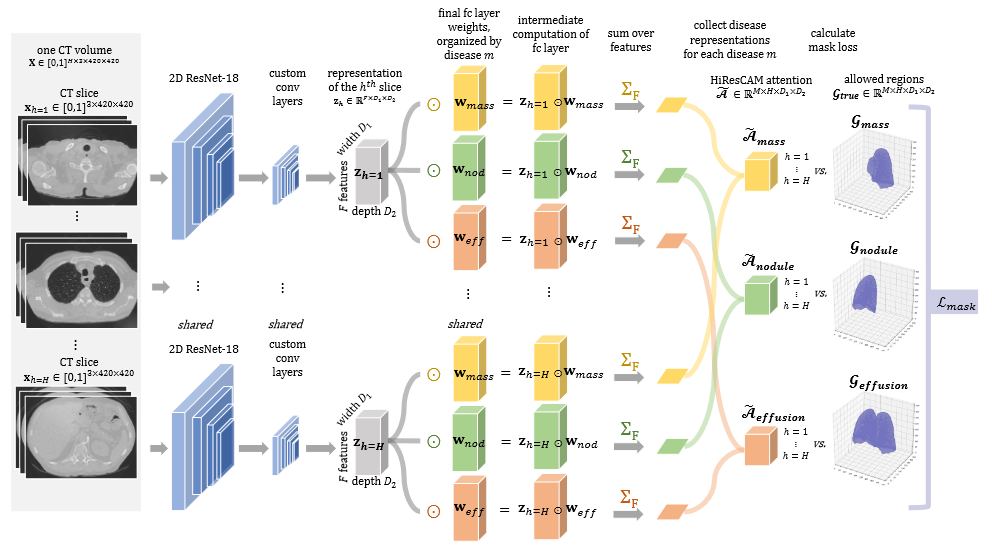
\includegraphics[scale=0.8]{../images/HiResCAM算法结构图.png}
		\caption{HiResCAM 算法结构图}
		\label{HiResCAM}
	\end{center}
\end{figure}

HiResCAM 算法和 GradCAM 算法的流程相似。其区别仅在于 HiResCAM 不对梯度取任何平均池化操作。而是直接将梯度和特征图进行元素级相乘来计算
热力图各像素的取值。
\begin{equation}
HCAM_c(i,j)=\sum_{k=1}^{K}\frac{\partial l^c}{\partial A_k}\cdot A_k(i,j)
\end{equation}
其中,$l^c$ 是第 $c$ 类的 logits,$A_k$ 是第 $k$ 个通道上的特征图,$K$ 是通道数。

和 GradCAM 使用的对梯度的全局平均池化相比,在 HiResCAM 中,模型可以更好地注意到特征大小的缩放和符号变化,
从而检测到更多的隐蔽特征。和自然图像相比,医学图像的分类依据为多种较隐蔽的特征而非少数几种明显特征。
这使得 HiResCAM 在医学图像上的效果较好,而在自然图像上效果差于 GradCAM。

\subsection{测试时增强平滑}
测试时增强平滑将输入的待检测图像进行水平翻转和亮度变换。求解所有增强图像和原始图像的热力图并将这些热力图的平均值作为
最后的输出。

测试时增强平滑可以使得热力图更加围绕着物体。

\subsection{主成分降噪平滑}
主成分降噪平滑将各种 CAM 算法得到的 CAM 热力图进行主成分分析,提取最重要的分量,从而实现热力图的降噪。 

主成分降噪平滑可以减少热力图的噪音。


\section{实验结果}
\subsection{实验环境}
本实验在本地笔记本电脑上进行,配置如表\ref{服务器配置}所示。
同时,为了使结果可复现,我们将随机数种子固定为 1024。我们还使用了 GPU 加速训练。
\begin{table}[H]
	\centering
	\caption{实验环境表}
	  \begin{tabular}{c|c|c}
		\toprule
	  \multirow{3}[0]{*}{硬件} & CPU   & 11th Gen Intel(R) Core(TM) i7-11800H @ 2.30GHz \\
			& 内存大小    & 16G \\
			& GPU   & NVIDIA GeForce RTX 3060 Laptop GPU \\\hline
	  \multirow{3}[0]{*}{软件} & 操作系统  & Windows 11 \\
			& 深度学习框架 & PyTorch 1.13.0 \\
			& IDE   & Vscode \\\bottomrule
	  \end{tabular}
	\label{服务器配置}
\end{table}

\subsection{结果}
我复现了上章中提到的所有 CAM 可解释性算法。同时获取了 LIME 的源代码并进行了改写,使之可以整合进实验代码中。
我们的基础模型采用了 PyTorch 框架下的 AlexNet 猫狗分类的模型。
我们使用了 3 张图片:一张为猫、一张为狗。一张同时存在猫和狗。我们用这些图片对实现的所有可解释性算法进行了测试。
在实验中我们分析的特征图是最后一层卷积层经 ReLU 和 MaxPool2d 之后的特征图。测试的结果如下。

\subsubsection{特征图}
三张图片的输出特征图各通道的可视化结果如图\ref{特征图1}、\ref{特征图2}和\ref{特征图3}所示。
\begin{figure}[H]
	\begin{center}
		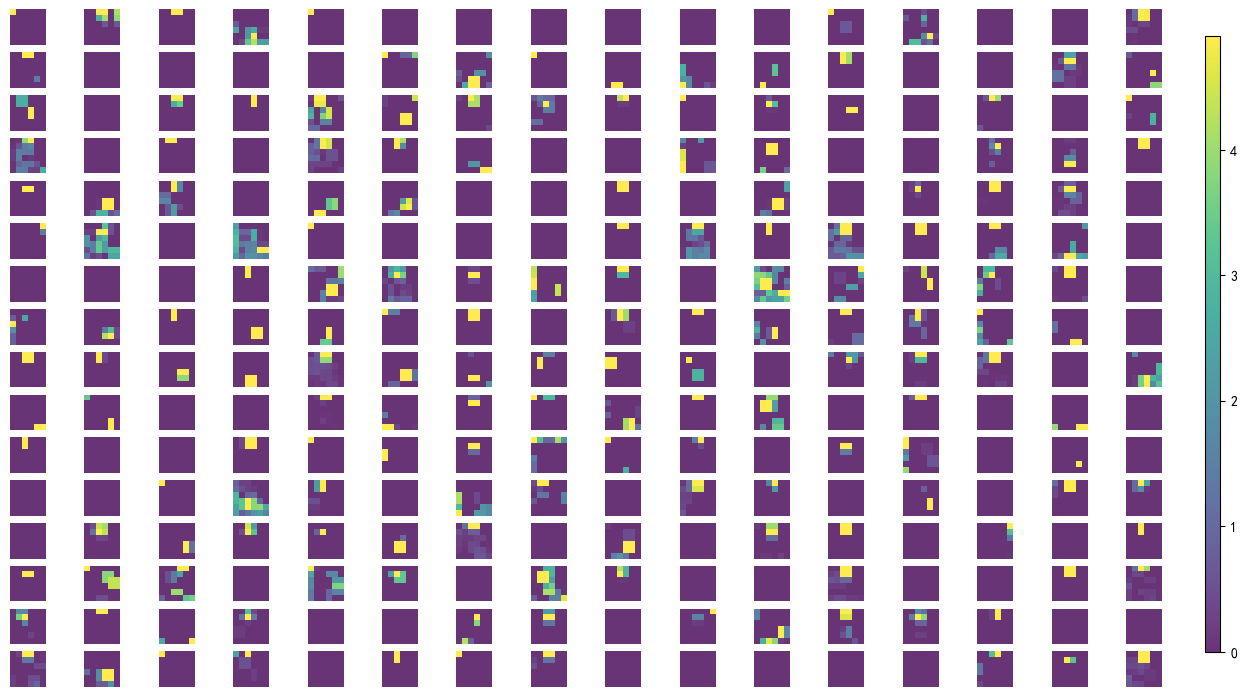
\includegraphics[scale=0.35]{../images/feature-map0.png}
		\caption{both 特征图}
		\label{特征图1}
	\end{center}
\end{figure}
\begin{figure}[H]
	\begin{center}
		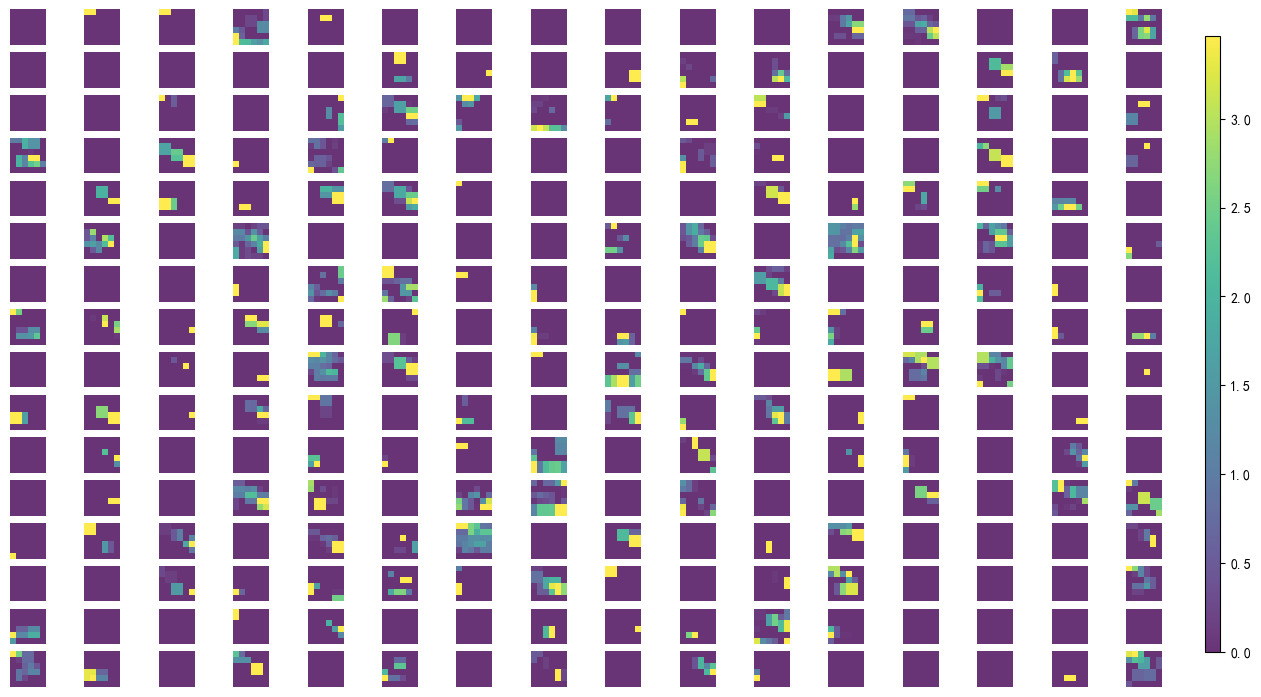
\includegraphics[scale=0.35]{../images/feature-map1.png}
		\caption{cat 特征图}
		\label{特征图2}
	\end{center}
\end{figure}
\begin{figure}[H]
	\begin{center}
		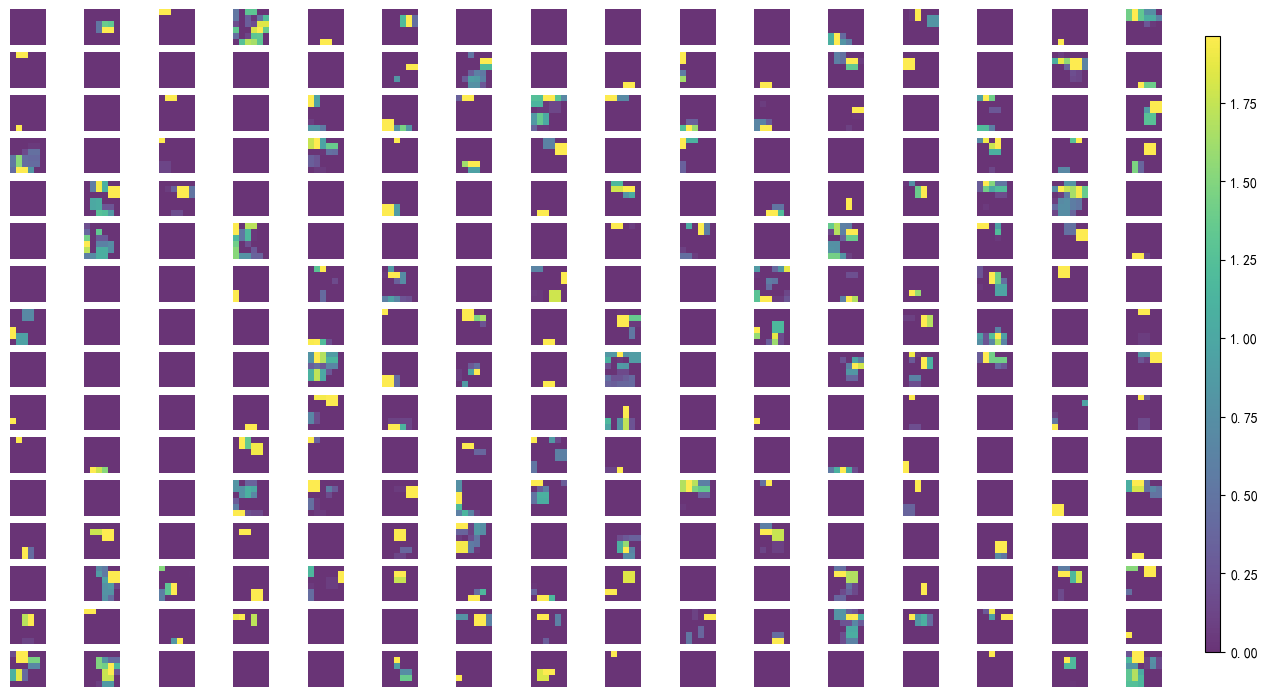
\includegraphics[scale=0.35]{../images/feature-map2.png}
		\caption{dog 特征图}
		\label{特征图3}
	\end{center}
\end{figure}

\subsubsection{LIME}
图\ref{LIME热力图}是 LIME 算法对三张图片生成的可视化结果。
\begin{figure}[H]
	\begin{center}
		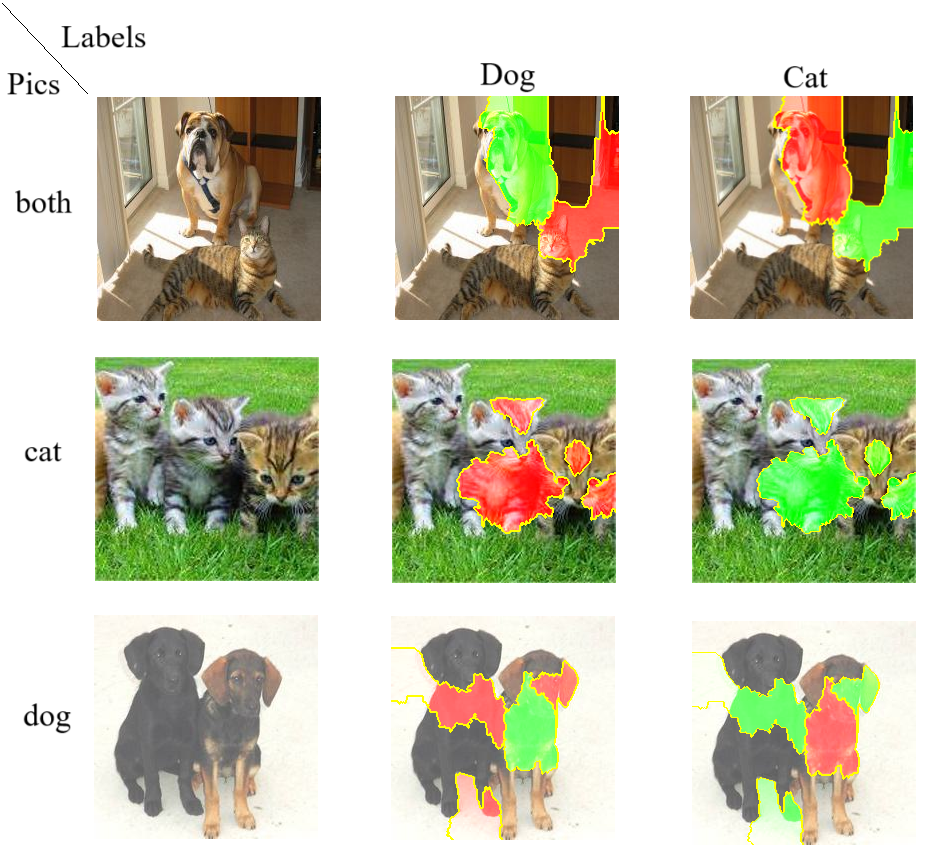
\includegraphics[scale=0.4]{../images/LIME热力图.png}
		\caption{LIME 热力图}
		\label{LIME热力图}
	\end{center}
\end{figure}

\subsubsection{CAMs}
当我们使用 GradCAM++ 可解释性分析算法时,
最终的 CAM 热力图如图 \ref{GradCAM++热力图}所示。
\begin{figure}[H]
	\begin{center}
		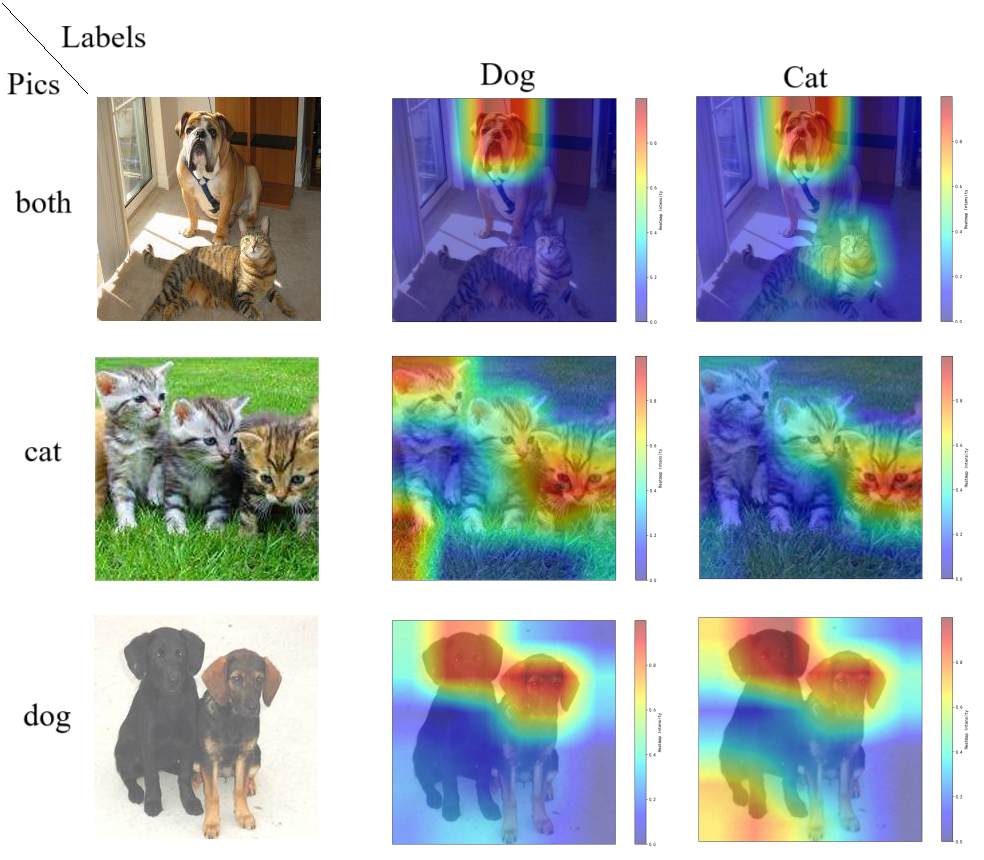
\includegraphics[scale=0.4]{../images/GradCAM++热力图.png}
		\caption{GradCAM++ 热力图}
		\label{GradCAM++热力图}
	\end{center}
\end{figure}

当我们使用 XGradCAM 可解释性分析算法时,
最终的 CAM 热力图如图 \ref{XGradCAM热力图}所示。
\begin{figure}[H]
	\begin{center}
		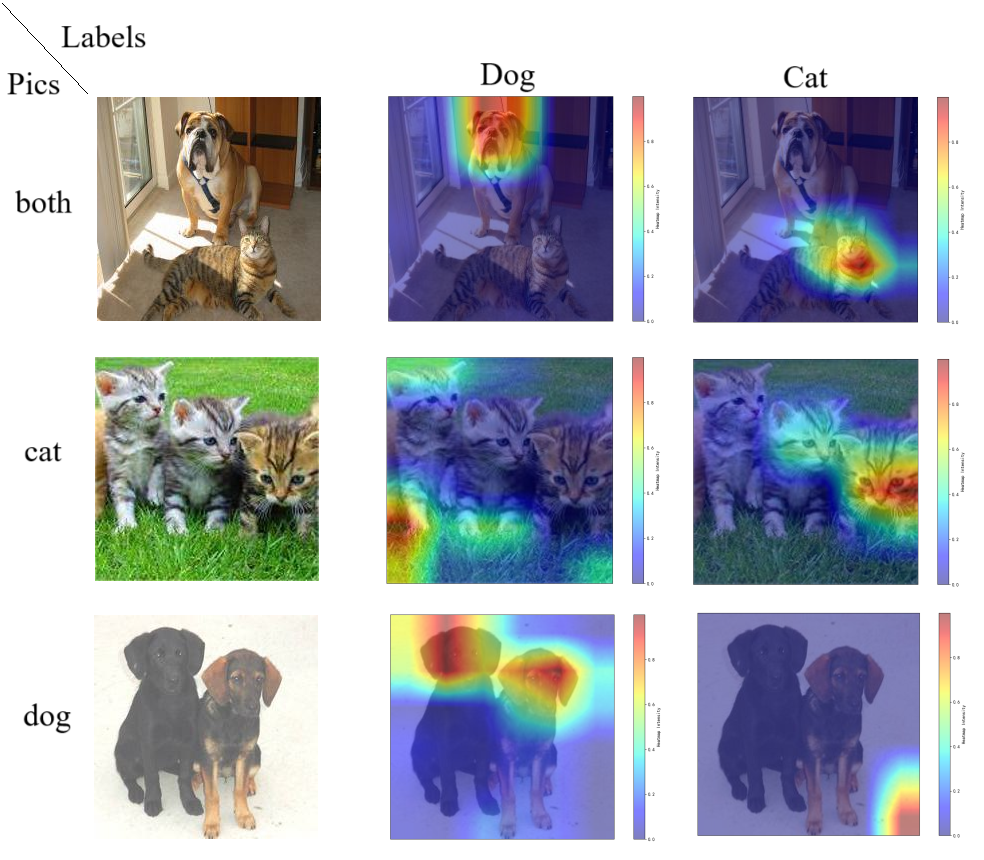
\includegraphics[scale=0.4]{../images/XGradCAM热力图.png}
		\caption{XGradCAM 热力图}
		\label{XGradCAM热力图}
	\end{center}
\end{figure}

当我们使用 ScoreCAM 可解释性分析算法时,
最终的 CAM 热力图如图 \ref{ScoreCAM热力图}所示。
\begin{figure}[H]
	\begin{center}
		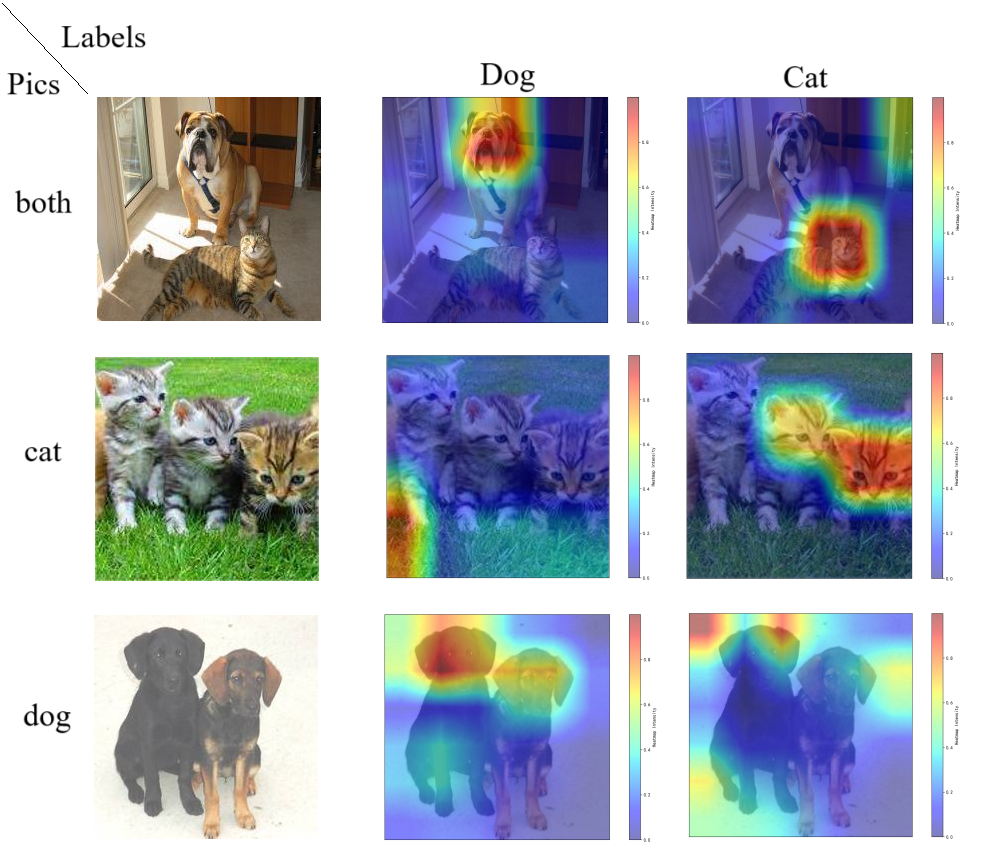
\includegraphics[scale=0.4]{../images/ScoreCAM热力图.png}
		\caption{ScoreCAM 热力图}
		\label{ScoreCAM热力图}
	\end{center}
\end{figure}

当我们使用 HiResCAM 可解释性分析算法时,
最终的 CAM 热力图如图 \ref{HiResCAM热力图}所示。
\begin{figure}[H]
	\begin{center}
		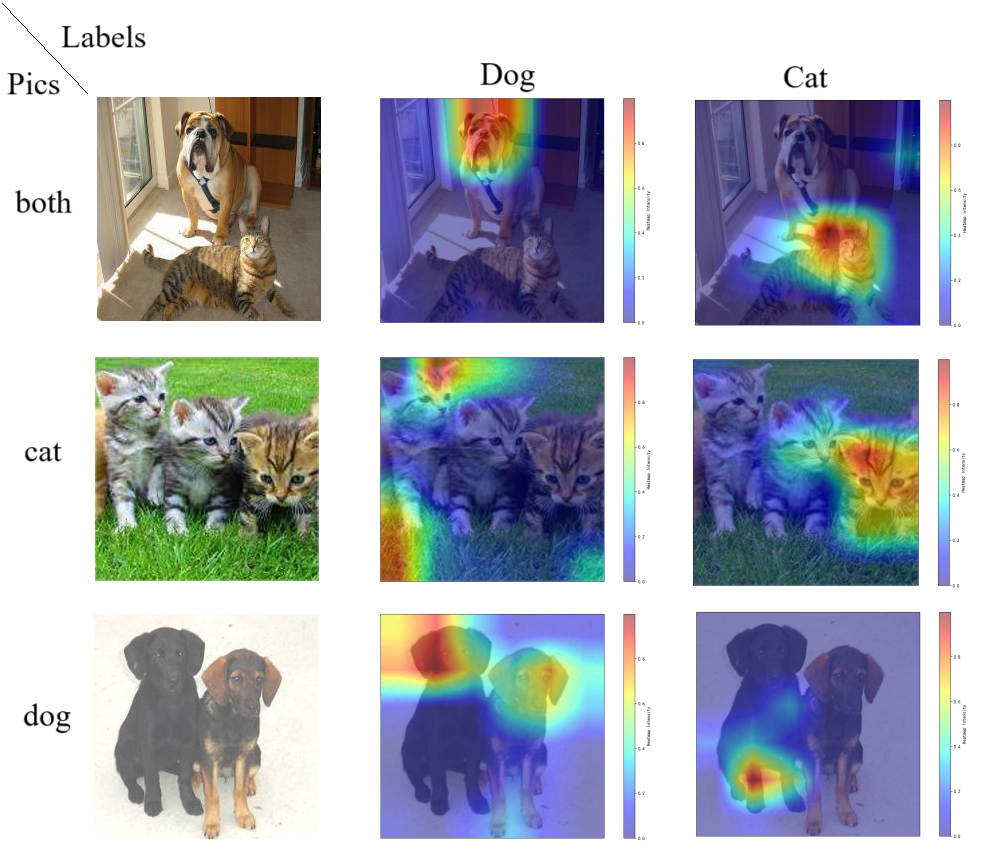
\includegraphics[scale=0.4]{../images/HiResCAM热力图.png}
		\caption{HiResCAM 热力图}
		\label{HiResCAM热力图}
	\end{center}
\end{figure}

\subsubsection{CAMs 平滑处理}
我们对每一种 CAM 模型都进行了无平滑、测试时增强平滑、主成分降噪平滑以及测试时增强平滑+主成分降噪平滑 4 种平滑模式的测试。
图\ref{平滑对比}展示了 4 种平滑选项的结果热力图差异。由于篇幅限制,本文仅展示 GradCAM 下的平滑结果对比。所有的平滑结果见附件中的 \emph{./results} 目录。
\begin{figure}[H]
	\begin{center}
		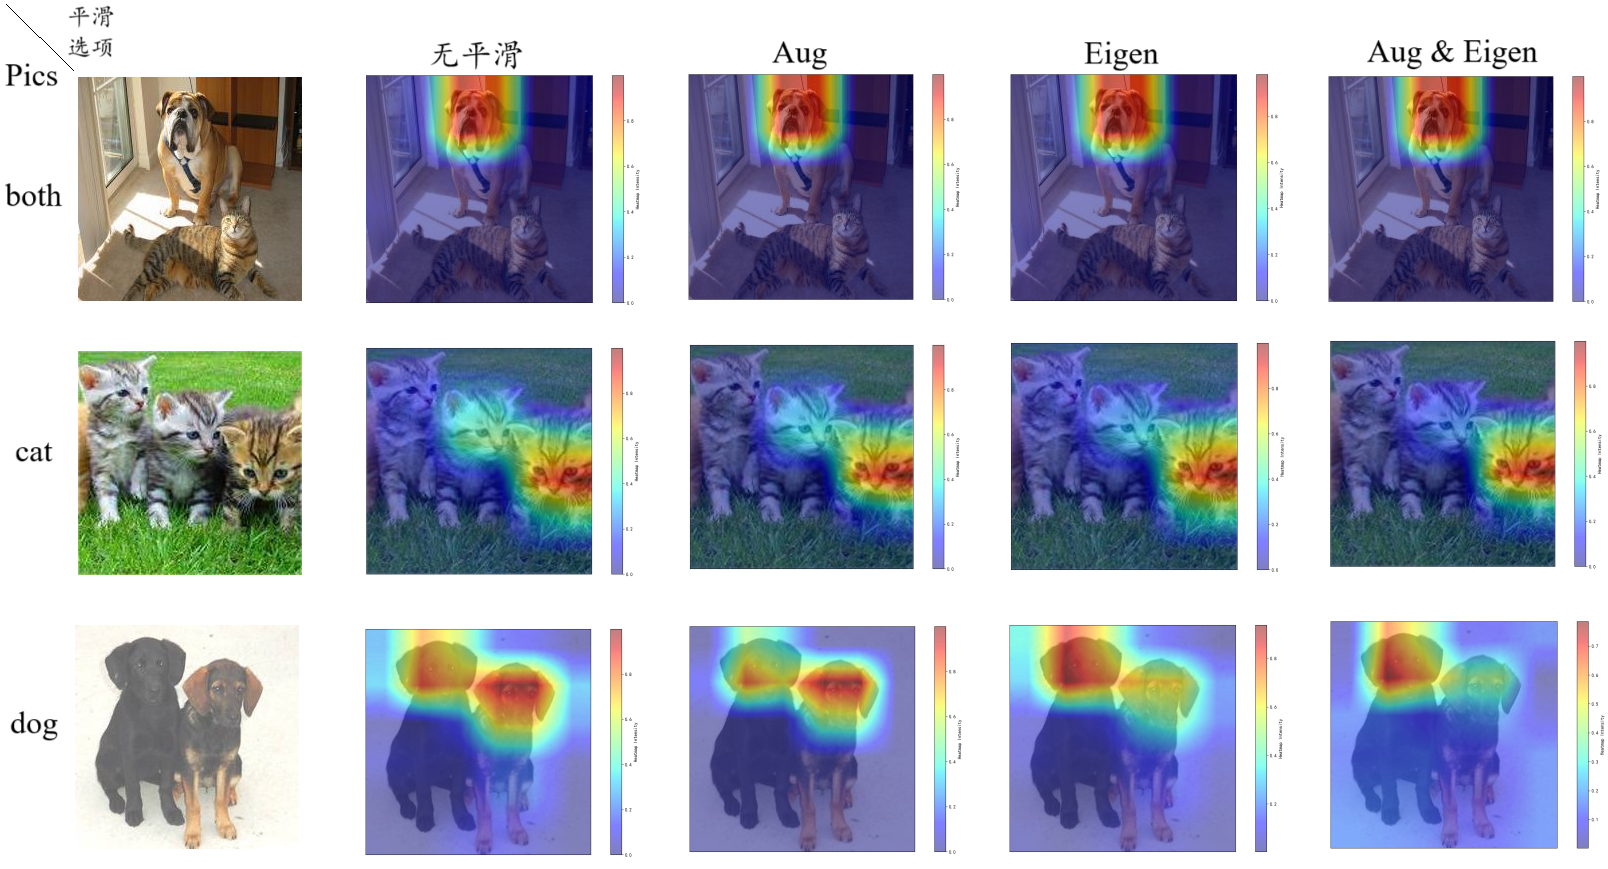
\includegraphics[scale=0.45]{../images/平滑对比.png}
		\caption{GradCAM 平滑结果热力图对比}
		\label{平滑对比}
	\end{center}
\end{figure}

\section{总结与讨论}
在这一章,我们主要对以上所述的几种不同的可解释性分析算法的实验结果进行讨论与分析。
\subsection{总述}
首先,我们对特征图进行简要分析。
最后一层卷积层的特征图表示输入图像的深层特征。
我们观察特征图的可视化结果\ref{特征图1}、\ref{特征图2}和\ref{特征图3},发现它们并不能为人类所直观地理解。
所以,我们只能通过 LIME,CAM 等可解释性分析算法来理解这些特征图的含义。

接着,我们对 LIME 算法的结果进行分析。
图\ref{LIME算法大致流程}中,绿色标识的区域是最有力支持当前标签的区域,而红色标识的区域是最有力支持当前标签的区域。
从图中我们可以看出,狗的面部特征最有力地支持了图像内容为狗的假设,最有力地反对了当前图像内容为猫的假设。所以,LIME 算法正确地对模型进行了解释。

最后,我们对 4 种 CAM 算法进行分析。
从图\ref{GradCAM++热力图}、\ref{XGradCAM热力图}、\ref{ScoreCAM热力图}以及\ref{HiResCAM热力图}中
我们可以看出 4 种 CAM 算法的结果差异不大,它们都成功显示了模型在进行分类时关注的图片区域。

对于 both 图片,我们发现模型在分类为狗时关注狗的面部,而分类为猫时
关注猫的面部。模型最终分类为狗的原因可能是狗的面部占据的面积大于猫的
面部占据的面积,而模型主要通过面部的特征来进行分类。

对于 cat 图片,我们发现模型最关注从左向右第三只小猫的面部,也关注了
中间的小猫面部,而几乎未关注从左向右第一只小猫。所以模型分类为猫。模型
对三只小猫的关注差异可能和它们面部的角度有关。小猫的正向面部相较于侧
向面部,含有更多猫的特征,所以更容易被模型所关注。由于这张图片中没有
狗,所以分类为狗时的热力图没有意义。

对于 dog 图片,我们发现模型关注了图片中两只狗的面部。所以模型分类为
狗。由于两只狗的面部全部是正向,含有的特征信息数量差异不大,所以模型同
时关注了它们。由于这张图片中没有猫,所以分类为猫时的热力图没有意义。
\subsection{可解释性算法优缺点对比}
\subsubsection{LIME}
和 CAM 算法相比,LIME 算法的一个显著优点是通用性强。LIME 算法可以解释包含文本、图像分类在内的几乎所有分类模型。
但是,由于 LIME 是一个局部解释模型,所以无法对极其复杂的非线性模型进行全局解释。
另外,LIME 算法需要重新训练一个线性模型,其时空开销较 CAM 算法大。

\subsubsection{GradCAM++}
GradCAM++ 算法作为一种 GradCAM 的改进算法,
解决了GradCAM 存在的难以检测全部同类物体和难以完全覆盖单一物体的问题。
此外,GradCAM++ 算法在图像描述生成、动作识别等任务的解释方面也具有优势。
然而,GradCAM++ 同样存在缺陷:缺乏明确的理论支持,例如不清楚为何可以使用像素级的加权平均作为每个特征的权重。

\subsubsection{XGradCAM}
XGradCAM 为 CAM 算法提供了清晰的数学解释,填补了 CAM 可视化方法本身在解释性方面的不足。
同时,它从公理的角度对 GradCAM 和 GradCAM++ 算法的有效性给出了合理的解释。
然而,基于梯度的 CAM 方法存在一些难以克服的问题,包括梯度的饱和性、梯度本身的不稳定性性以及梯度消失的影响。
这些问题导致在 GradCAM 中一些特征图得到了较高的权重,但其在网络中的响应却较低,而一些权重较低的特征图却获得了较高的置信度。

\subsubsection{ScoreCAM}
ScoreCAM 算法摆脱了对梯度的依赖,仅需要前向传播即可计算出 CAM 热力图。
这样以来,在规避了由梯度引发的可解释性问题的同时,还减小了计算开销。

\subsubsection{HiResCAM}
HiResCAM 是医学图像处理领域中对 GradCAM 的改进。改进使得 HiResCAM 检测隐蔽特征的能力增强,更适合 3D 医学图像。
但是其在自然图像上的效果差于 GradCAM 算法。

\subsection{平滑方法对比}
从图\ref{平滑对比}中我们可以看出,两种平滑方法都起到了使热力图更加集中的作用。
当两种平滑方法都使用时,集中效果最好。
但是,平滑方法加剧了各种 CAM 算法中存在的难以检测全部同类物体和难以完全覆盖单一物体的问题,
并且忽略了一些较隐蔽的特征。所以,当在目标由多种隐蔽特征而非少数明显特征区分的场合使用可解释性算法时,
如在医学图像处理时使用 HiResCAM 时,不宜采用任何平滑方法。

\section{实验代码简述}
在本章中,我们简要介绍实验代码的构成。更具体的介绍请见 ReadMe.md 文件。

工作目录中存在 5 个文件和 2 个目录。整个工作目录的结构如下。
\begin{figure}[H]
	\begin{center}
		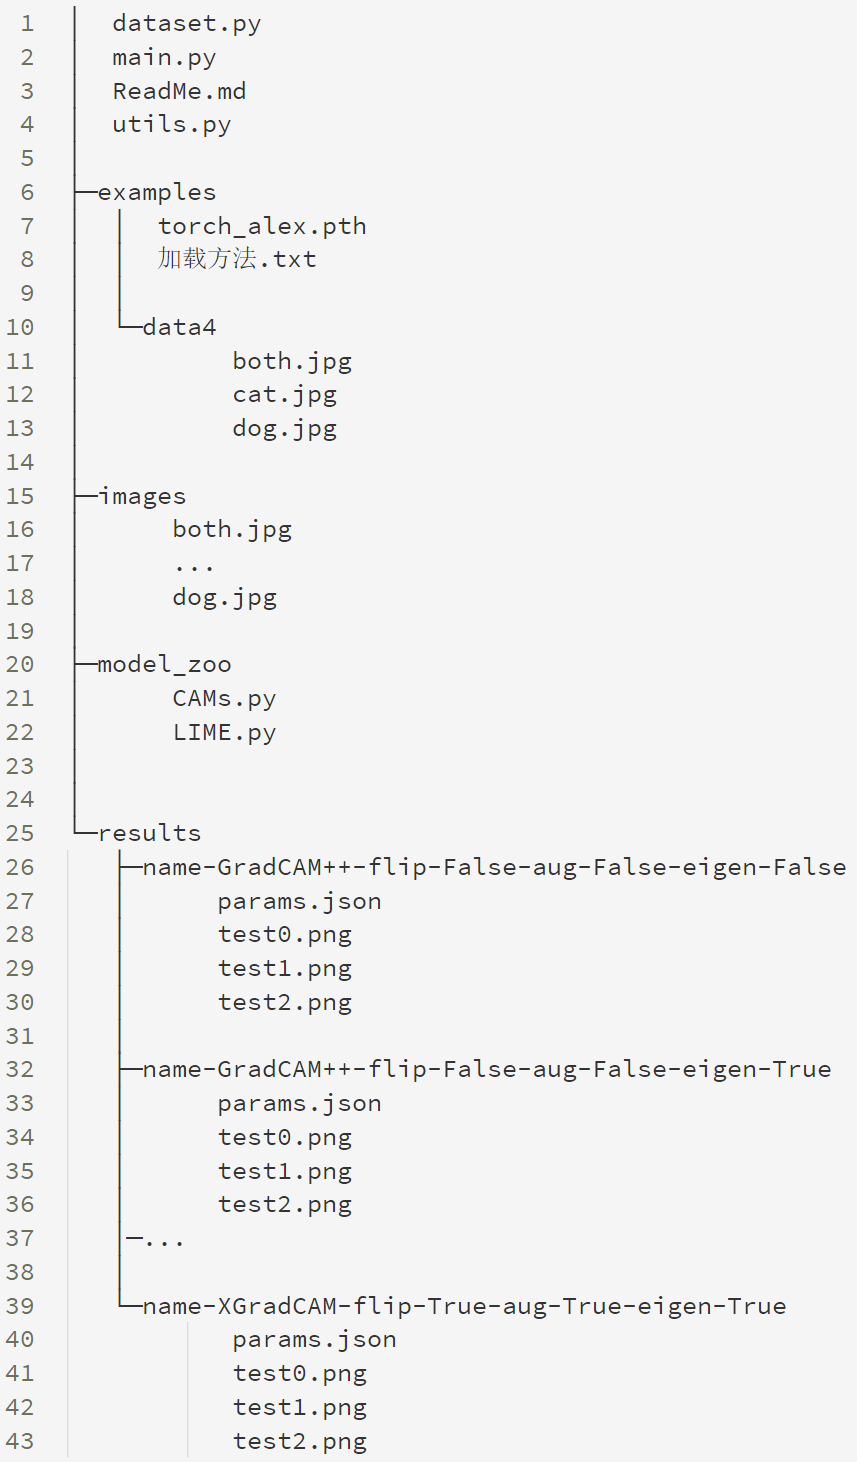
\includegraphics[scale=0.5]{../images/tree.png}
		\caption{工作目录的结构}
	\end{center}
\end{figure}

其中,dataset.py 中含有数据预处理的相关函数。
ReadMe.md 中介绍了如何对模型进行训练和测试。main.py 是实现可解释性计算的主程序。
utils.py 中含有一些工具函数。各函数和类的源代码均含有详细的注释,方便使用者了解其完成的工作。
images 目录存放所有绘制的图像。model\_zoo 目录存放 CAM 和 LIME 的网络结构。
results 目录存放了各种超参数下的可视化结果热力图。

% \nocite{*}

\bibliography{Experimental_Report}

\end{document}